% Appendix E

\chapter{Zapojenie Q-C metódy a metodika merania parazitných kapacít.} % Main appendix title

\label{app:AppendixE} % For referencing this appendix elsewhere, use \ref{AppendixA}

\lhead{Appendix E. \emph{Zapojenie Q-C metódy a metodika merania parazitných kapacít}} % This is for the header on each page - perhaps a shortened title

Autori metódy uvádzajú v \cite{App.2,App.3,App.4} podrobný popis
analógovej aj digitálnej implementácie Q-C metódy.  V oboch
implementáciách na meranie kapacity používajú prístroj PAR 410,
namiesto ktorého sme v našom prípade použili prístroj HP4280a. Okrem
potrebných detailov týkajúcich sa zapojenia metódy autori popisujú
metodiku merania parazitných kapacit, prípadne ich elimináciu. Treba
spomenúť, že pri meraní a eliminácii parazitných kapacít možno
postupovať viacerými postupmi. V ďalšom popíšeme zapojenie, ktoré sme
použili, ako aj zvolený postup merania parazitných kapacít. Avšak pre
dokonalé zvládnutie tejto komplexnej metódy je potrebné zoznámenie sa
s podrobným popisom v \cite{App.2,App.3,App.4}.

\begin{figure}[h!]\centering
%\framebox[10cm]{\rule{0cm}{3cm}}
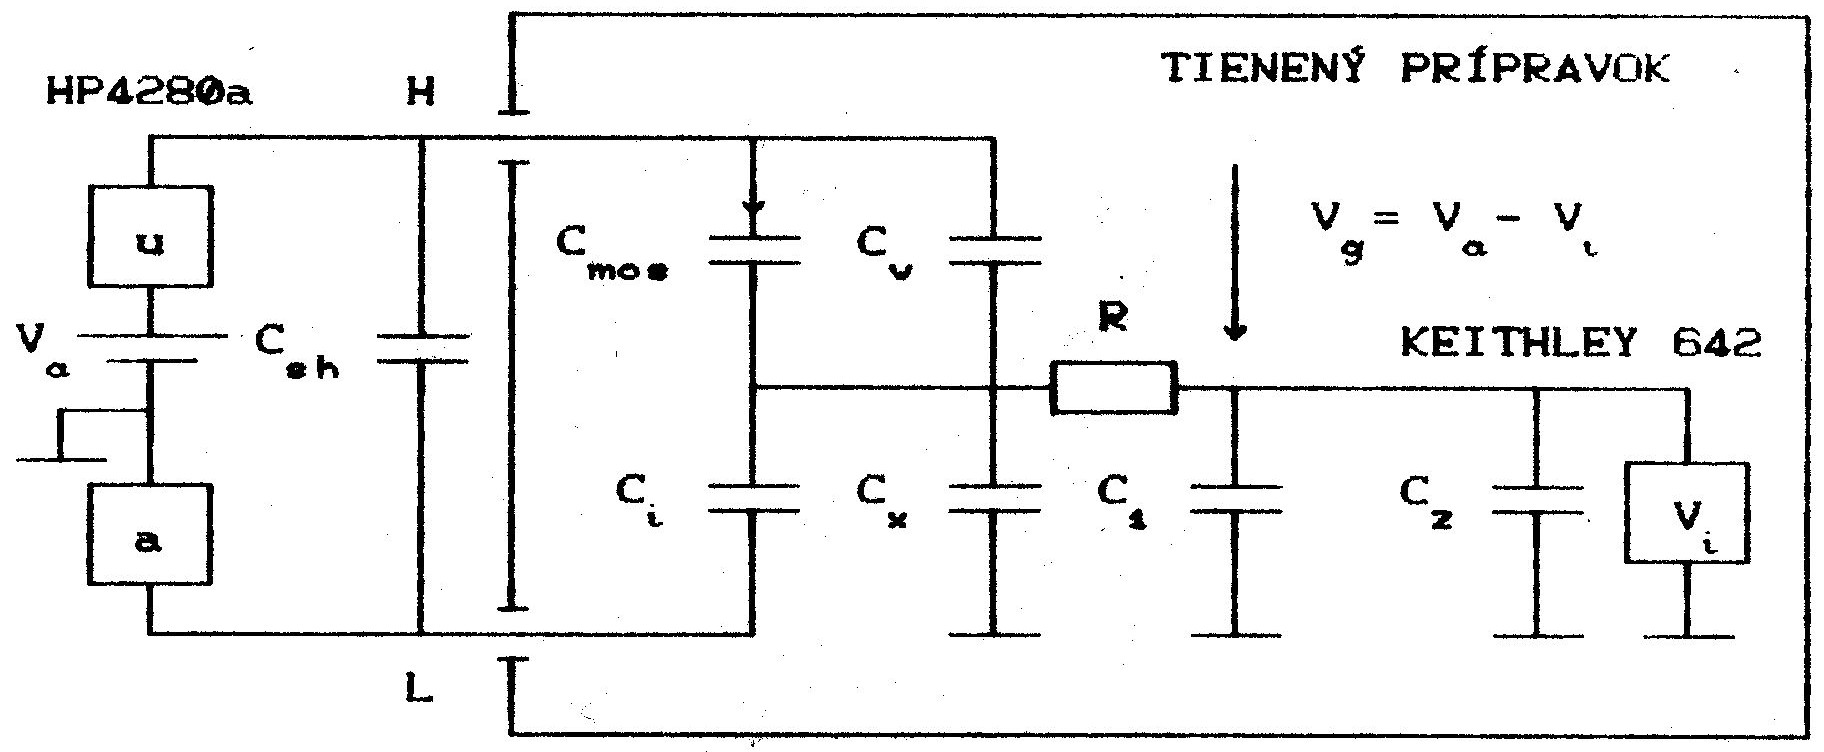
\includegraphics{Figures/fig-app-1.eps}
\captionsetup{justification=raggedright, singlelinecheck=false}
\caption[Zapojenie Q-C metódy implementované na KME EF
  SVŠT.]{Zapojenie Q-C metódy implementované na KME EF SVŠT.}
\label{fig:App.1}
\end{figure}

\par Na obrázku \ref{fig:App.1} je znázornené detailné zapojenie
pracovného stolíka a meracích prístrojov Q-C metódy. V ľavej časti
obrázku je znázornený merací prístroj HP4280a, ktorý na našej schéme
pozostáva zo zdroja jednosmerného napätia $V_a$, ktorým je meraná
štruktúra privedená do požadovaného stavu, zdroja vysokofrekvenčného
signálu (označeného u) a ampérmetra (označeného a).  Kapacita $C_{sh}$
predstavuje parazitnú kapacitu prívodných vodičov, ktorú možno
eliminovať priamo pomocou meracieho prístroja HP4280a, a preto ju
ďalej nebudeme uvažovať. $C_{mos}$ je kapacita meranej štruktúry a $C_i$
predstavuje napäťovo nezávislý kondenzátor. Kapacita $C_w$ znázorňuje
parazitnú kapacitu medzi stolíkom, na ktorom sa nachádza meraná
šruktúra a zdvihnutým hrotom sondy. $C_x$ označuje parazitnú kapacitu
medzi spoločným bodom zapojenia kondenzátorov (ďalej len spoločný bod)
a zemou.  $C_1$ predstavuje parazitnú kapacitu prívodného vodiča k
voltmetru a $C_2$ označuje vstupnú kapacitu voltmetra.  Uvedené
kapacity $C_1$ a $C_2$ tvoria spolu s odporom R dolnopriepustný
filter, ktorý odizoluje voltmeter od vysokofrekvenčného signálu,
generovaného prístrojom HP4280a. Problémom vysokofrekvenčného merania
je skutočnosť, že ampérmeter prístroja HP4280a nemeria zložku prúdu
tečúcu zo spoločného bodu cez kondenzátory $C_x$, $C_1$ a $C_2$ na
zem. Uvedenú skutočnosť treba zohľadniť pri vyhodnotení
vysokofrekvenčného merania. Pre konečné vyhodnotenie nameraných údajov
je potrebné vyriešiť následovné úlohy:

\begin{itemize}
\item určenie kapacity $C_i$
\item určenie parazitnej kapacity $C_w$
\item určenie parazitnej kapacity $Cx$
\item určenie kapacity $C_{iLF}  = C_i  + C_1  + C_2$
\item korekcia meranej vysokofrekvenčnej kapacity $C_m$ vzhľadom na prúd
  tečúci cez $C_x + C_1 + C_2$ na zem.
\end{itemize}


\section{Určenie parazitnej kapacity $C_w$.}\label{sec:E.1}

Podrobný popis metodiky merania parazitnej kapacity $C_w$ je v dodatku
2. literatúry \cite{App.2}. V našom experimente sme spomenutú metodiku
modifikovali spôsobom, ktorý viedol k väčšej reprodukovatelnosti
výsledkov. Tento postup popíšeme.

\begin{enumerate}
\item pripojíme štruktúru MOS a pri $V_a = 0$ na okamih uzemníme
  spoločný bod, aby sme zaistili nulový vonkajši náboj na
  kondenzátoroch.
\item napätím $V_a$ privedieme štruktúru MOS do akumulácie a
  odčítame hodnoty $V_a = V_{a0}$ a $V_i = V_{i0}$ .
\item privedieme štruktúru MOS vyšším napätím $V_a$ do akumulácie a
  odčítame hodnoty $V_a = V_{a1}$ $V_i = V_{i1}$. Zo zákona zachovania
  náboja vyplýva
\begin{equation}\label{eq:E.1}
(C_{ox} + C_w)(V_{g1} - V_{g0}) = (C_{iLF} + C_x)(V_{i1} - V_{i0})
\end{equation}
\item nastavíme $V_a=0$, na okamih uzemníme spoločný bod a zdvihneme
  hrot sondy práve tak, aby sme prerušili kontakt.
\item nastavíme $V_a \neq 0$ a odčítame hodnoty $V_a = V_{a2}$ $V_i =
  V_{i2}$.
\item zvýšime napätie $V_a$ a odčítame hodnoty $V_a = V_{a3}$ $V_i =
  V_{i3}$. Zo zákona zachovania náboja vyplýva
\begin{equation}\label{eq:E.2}
C_w (V_{g3} - V_{g2}) = (C_{iLF} + C_x)(V_{i3} - V_{i2})
\end{equation}
\item porovnaním vzťahov \ref{eq:E.1} a \ref{eq:E.2} dostaneme výraz
  pre výpočet kapacity $C_w$, ktorú môžeme vyhodnotiť za predpokladu,
  že poznáme kapacitu oxidovej vrstvy štruktúry MOS.
\begin{equation}\label{eq:E.3}
C_w = C_{ox} \frac{1} {\frac {\frac{V_{g3}-V_{g2}}{V_{g1}-V_{g0}}} {\frac{V_{i3}-V_{i2}}{V_{i1}-V_{i0}}} -1}
\end{equation}
\end{enumerate}


\section{Určenie parazitnej kapacity $C_x$.}\label{sec:E.2}

V dodatku 10 literatúry \cite{App.4} sa nachádza popis priameho
merania parazitnej kapacity $C_x$.  Avšak experimentálne výsledky
ukazujú, že toto meranie je zaťazené veľkou chybou a jeho
reprodukovateľnosť je malá. Preto sme zvolili v našom experimente
postup, ktorého princíp je načrtnutý v dodatku 5 literatúry
\cite{App.4}. Ako možno vidieť v dodatku \ref{sec:E.4},
vysokofrekvenčná kapacita štruktúry MOS $C_{mos}$ je funkciou
parazitnej kapacity $C_x$, ktorú chceme určiť. V akumulácii musí
platiť $C_{mos} = C_{ox}$, čo môžeme dosiahnuť vhodnou variáciou
hodnoty $C_x$ . V našom vyhodnotení dát nameraných Q-C metódou sme na
variáciu hodnoty $C_x$ použili metódu delenia intervalov.


\section{Určenie kapacity $C_{iLF}$.}\label{sec:E.3}

V dodatku 10 literatury \cite{App.4} sa nachádza popis priameho
merania parazitnej kapacity $C_{iLF}$. Avšak podobne ako pri meraní
$C_x$ experimentálne výsledky ukazujú, že toto meranie je zaťažené
veľkou chybou. Preto sme zvolili postup, ktorý vychádza z podmienky,
že nízkofrekvenčná a vysokofrekvenčná kapacita štruktúry MOS musia mať
tú istú hodnotu v akumulácii. Určenie $C_{iLF}$ potom vychádza z
následujúceho vzťahu

\begin{equation}\label{eq:E.4}
\frac{\delta}{\delta C_{iLF}} \sum\limits_{j} \bigg[C_{mos}^{LF}(j) - C_{mos}^{HF}(j)\bigg]^2 = 0
\end{equation}

kde horeuvedenú sumáciu vykonávame pre body namerané v
akumulácii. Popis odvodenia vzťahu pre výpočet $C_{iLF}$ je v dodatku
4 literatúry \cite{App.4} a tu uvedieme len jeho konečnú podobu.

\begin{equation}\label{eq:E.5}
C_{iLF} = \frac{\sum\limits_{j} {\Bigg[C_{mos}^{HF}(j)+C_{w}\Bigg]\Bigg[\frac{dV_i}{dV_g}\Bigg]_j}}
{\sum\limits_{j} \Bigg[\frac{dV_i}{dV_g}\Bigg]_j}
\end{equation}
%C_{iLF} = \frac{\sum_{j}\Big[C_{mos}^{HF}(j)+C_{w}\Big]\Big[\frac{dV_i}{dV_g}\Big]_j}
%{\sum_{j}\Big[\frac{dV_i}{dV_g}\Big]}

Treba upozorniť, že uvedený postup má tú výhodu, že jeho použitie
zaručuje koincidenciu nízkofrekvenčnej a vysokofrekvenčnej kapacitnej
závislosti štruktúry MOS v akumulácii, čo predstavuje dobrý základ pre
výpočet pascí rozhrania z uvedených dvoch kapacitných závislostí.


\section{Korekcia vysokofrekvenčnej kapacity $C_m$.}\label{sec:E.4}

V dodatku 1 literatúry \cite{App.2} je uvedená analýza zapojenia Q-C
metódy z pohľadu vysokofrekvenčného merania. Tu uvedieme jej hlavnú
myšlienku.

\begin{figure}[h!]\centering
%\framebox[10cm]{\rule{0cm}{3cm}}
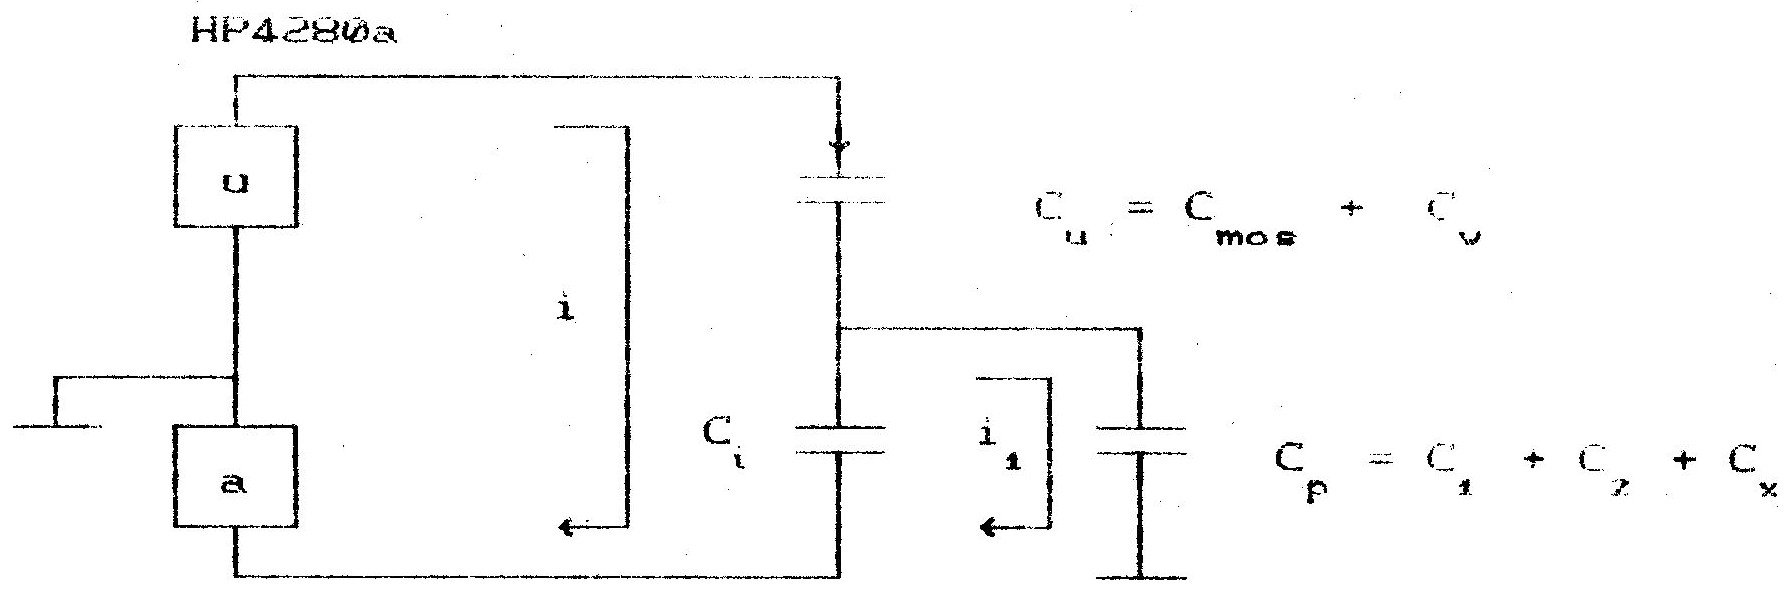
\includegraphics{Figures/fig-app-2.eps}
\captionsetup{justification=raggedright, singlelinecheck=false}
\caption[Ekvivalentné zapojenie Q-C metódy pre vysokofrekvenčné
  meranie]{Ekvivalentné zapojenie Q-C metódy pre vysokofrekvenčné
  meranie.}
\label{fig:App.2}
\end{figure}

Ako vidieť z obrázku \ref{fig:App.2} ampérmeter prístroja HP4280a
nemeria prúd $i_1$ tečúci cez kondenzátor $C_p$ . Kapacitu $C_m$,
ktorú pomocou tohoto prístroja nameriame, môžeme vyjadriť vzťahom

\begin{equation}\label{eq:E.6}
C_m = \frac{C_{u} C_{iHF}} {C_{iHF}+C_{u}+C_{p}}
\end{equation}

V kapitole \ref{sec:3.3} sú uvedené vzťahy pre výpočet
vyskofrekvenčnej kapacity štruktúry MOS.  Aby výsledky, získané zo
vzťahov \ref{eq:3.3} neboli ovplyvnené uvedenou skutočnosťou, treba
urobiť následujúce korekcie (podľa dodatku 1 literatúry \cite{App.4})

\begin{equation}\label{eq:E.7}
C_{iHF}=C_{iHF}k, \qquad G_{m}=G_{m}k, \qquad C_{m}=C_{m}k
\end{equation}

,kde

\begin{equation}\label{eq:E.8}
k = 1 + \frac{C_x}{C_{iHF}}
\end{equation}
